\section{Thuật toán Quick Search}

\subsection{Đặc điểm chính}
Quick Search là một thuật toán tìm kiếm chuỗi được đề xuất bởi Daniel M. Sunday như một biến thể đơn giản hóa của thuật toán Boyer-Moore. Thuật toán chỉ sử dụng heuristic bad-character để xác định khoảng dịch chuyển của mẫu, nhờ đó cấu trúc cài đặt trở nên ngắn gọn và dễ triển khai hơn so với Boyer-Moore đầy đủ.

Mặc dù có độ phức tạp thời gian trong trường hợp xấu nhất là bậc hai, Quick Search thường cho hiệu năng rất tốt trong thực tế, đặc biệt đối với các mẫu ngắn và bảng chữ cái lớn. Nhờ cơ chế dịch chuyển dựa trên ký tự ngay sau cửa sổ hiện tại, thuật toán thường đạt được khoảng dịch chuyển lớn và giảm số lần thử khớp không cần thiết.

Thuật toán có các đặc điểm sau:

\begin{itemize}
    \item là phiên bản đơn giản hóa của thuật toán Boyer-Moore;
    \item chỉ sử dụng phép dịch chuyển bad-character;
    \item dễ cài đặt;
    \item giai đoạn tiền xử lý có độ phức tạp thời gian $O(m + \sigma)$ và độ phức tạp không gian $O(\sigma)$;
    \item giai đoạn tìm kiếm có độ phức tạp thời gian $O(mn)$;
    \item hoạt động rất nhanh trong thực tế đối với mẫu ngắn và bảng chữ cái lớn.
\end{itemize}

\subsection{Mô tả thuật toán}

Thuật toán Quick Search chỉ sử dụng bảng dịch chuyển bad-character 
(xem thuật toán Boyer-Moore). Sau mỗi lần thử mà cửa sổ được đặt trên 
đoạn văn bản $y[j \dots j + m - 1]$, độ dài dịch chuyển luôn lớn hơn hoặc 
bằng 1. Do đó, ký tự $y[j + m]$ chắc chắn sẽ tham gia vào lần thử kế tiếp, vì vậy 
ký tự này có thể được sử dụng để tính toán phép dịch chuyển bad-character cho 
lần thử hiện tại.

Phép dịch chuyển bad-character trong thuật toán này được 
điều chỉnh nhẹ để xét thêm ký tự cuối cùng của mẫu 
$x$ như sau: với mọi ký tự $c in \Sigma$,

\[
qsBc[c] =
\begin{cases}
\min \{\, i \mid 0 < i \leq m \text{ và } x[m-i] = c \,\},
& \text{nếu } c \text{ xuất hiện trong } x; \\

m + 1,
& \text{ngược lại.}
\end{cases}
\]

(Cải tiến này được đề xuất bởi Darko Brljak.)

Giai đoạn tiền xử lý của thuật toán có độ phức tạp thời gian $O(m + \sigma)$ và 
độ phức tạp không gian $O(\sigma)$.

Trong giai đoạn tìm kiếm, các phép so sánh giữa ký tự của mẫu và văn bản 
trong mỗi lần thử có thể được thực hiện theo bất kỳ thứ tự nào. Mặc dù giai 
đoạn tìm kiếm có độ phức tạp thời gian bậc hai trong trường hợp xấu nhất, thuật 
toán vẫn cho hiệu năng rất tốt trong thực tế.


\subsection{Cài đặt bằng C++}

\begin{verbatim}
#include <iostream>
#include <vector>
#include <string>

using namespace std;

const int ASIZE = 256;

/* Preprocessing: Quick Search Bad Character Table */
void preQsBc(const string &pat, vector<int> &qsBc) {
    int m = pat.length();

    qsBc.assign(ASIZE, m + 1);

    for (int i = 0; i < m; ++i) {
        qsBc[(unsigned char)pat[i]] = m - i;
    }
}

/* Quick Search Algorithm */
void QuickSearch(const string &pat, const string &txt) {
    int m = pat.length();
    int n = txt.length();

    vector<int> qsBc;

    /* Preprocessing */
    preQsBc(pat, qsBc);

    /* Searching */
    int j = 0;

    while (j <= n - m) {
        int i = 0;

        while (i < m && pat[i] == txt[j + i]) {
            ++i;
        }

        if (i == m) {
            cout << "Pattern found at index: " << j << endl;
        }

        if (j + m < n) {
            j += qsBc[(unsigned char)txt[j + m]];
        } else {
            break;
        }
    }
}

int main() {
    string text = "ABAAABCDABCABC";
    string pattern = "ABC";

    QuickSearch(pattern, text);

    return 0;
}
\end{verbatim}

\subsection{Kiểm nghiệm thuật toán}
\textbf{Pha tiền xử lý:}

\begin{center}
    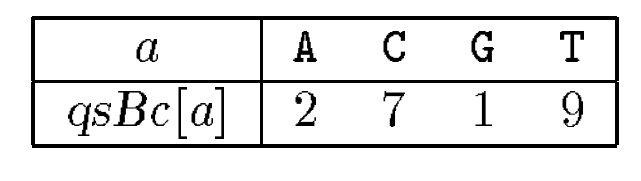
\includegraphics[width=10cm]{Images/2026-05-18-10-01-24.png}
\end{center}

Bảng $qsBc$ được sử dụng bởi thuật toán Quick Search.

\textbf{Pha tìm kiếm:}

Lần 1:

\begin{center}
    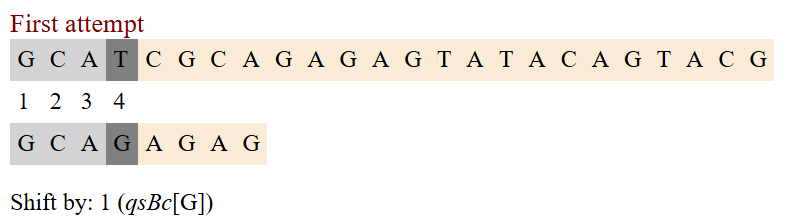
\includegraphics[width=10cm]{Images/2026-05-18-10-02-42.png}
\end{center}

Lần 2:

\begin{center}
    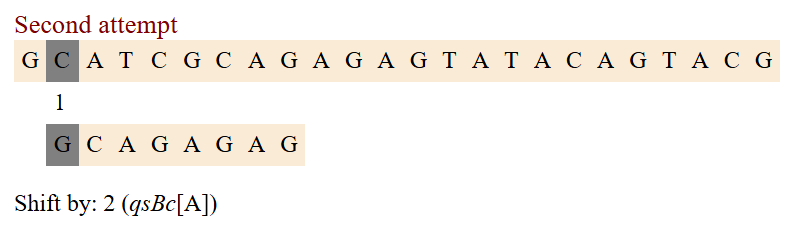
\includegraphics[width=10cm]{Images/2026-05-18-10-03-03.png}
\end{center}

Lần 3:

\begin{center}
    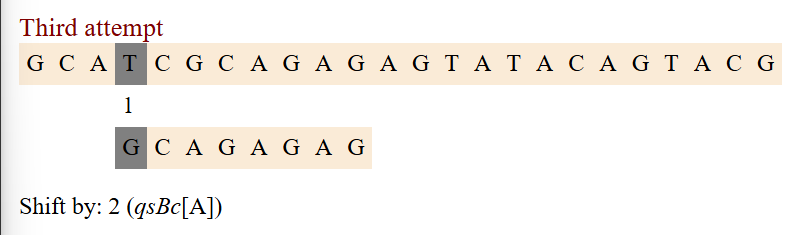
\includegraphics[width=10cm]{Images/2026-05-18-10-03-22.png}
\end{center}

Lần 4:

\begin{center}
    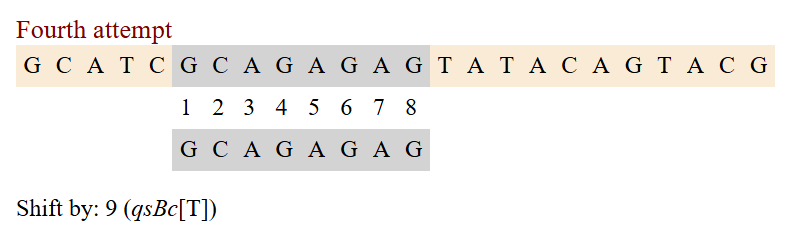
\includegraphics[width=10cm]{Images/2026-05-18-10-03-39.png}
\end{center}

Lần 5:

\begin{center}
    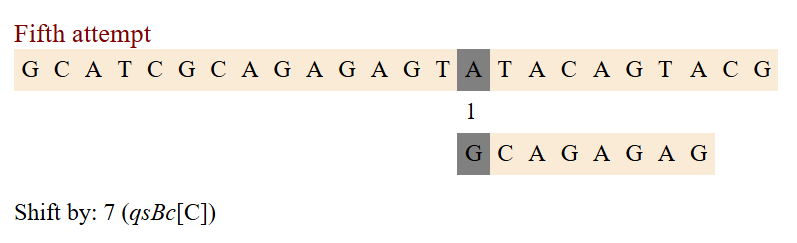
\includegraphics[width=10cm]{Images/2026-05-18-10-03-53.png}
\end{center}

Thuật toán Quick Search thực hiện 15 lần so sánh chuỗi trong ví dụ trên.


